\chapter*{Appendix A: Key Code Snippets}
\addcontentsline{toc}{chapter}{Appendix A: Key Code Snippets}
\markboth{APPENDIX A: KEY CODE SNIPPETS}{APPENDIX A: KEY CODE SNIPPETS}
\begin{spacing}{1.3}

\section*{A.1 Asynchronous Market Auction Sector Cost Computation}
The following Python implementation calculates the normalized bidding cost for drone $D_j$ across candidate spatial search sector $S_i$:

\begin{verbatim}
def compute_bidding_cost(drone_state, sector_polygon, w=(0.5, 0.3, 0.2)):
    """
    Computes marginal cost for drone Dj to bid on sector Si.
    w[0]: Distance weight, w[1]: Battery penalty weight, w[2]: Hazard factor
    """
    d_transit = np.linalg.norm(drone_state.position[:2] - sector_polygon.centroid)
    d_norm = d_transit / drone_state.max_mission_range
    
    battery_penalty = 1.0 - (drone_state.battery_pct / 100.0)
    hazard_penalty = sector_polygon.hazard_index  # Normalized 0.0 to 1.0
    
    cost = (w[0] * d_norm) + (w[1] * battery_penalty) + (w[2] * hazard_penalty)
    return float(cost)
\end{verbatim}

\section*{A.2 Embedded INT8 ONNX Runtime Inference Loop}
The following execution daemon processes incoming camera frames, performs letterboxing, and runs INT8 neural inference on the companion computer:

\begin{verbatim}
import cv2, onnxruntime as ort, numpy as np

session = ort.InferenceSession("models/yolov8n_int8.onnx", 
                               providers=["CPUExecutionProvider"])
input_name = session.get_inputs()[0].name

def detect_victims(frame, conf_threshold=0.25):
    # Letterbox resize to 640x640 and normalize to [0, 1]
    resized = cv2.resize(frame, (640, 640))
    blob = np.expand_dims(resized.transpose(2, 0, 1)/255.0, axis=0).astype(np.float32)
    
    outputs = session.run(None, {input_name: blob})[0]
    detections = []
    for pred in outputs[0]:
        conf = pred[4]
        if conf >= conf_threshold and int(pred[5]) == 0:  # Class 0: Person
            detections.append(pred[:4])
    return detections
\end{verbatim}

\end{spacing}

\clearpage
\chapter*{Appendix B: Additional Results and Visualizations}
\addcontentsline{toc}{chapter}{Appendix B: Additional Results and Visualizations}
\markboth{APPENDIX B: ADDITIONAL RESULTS}{APPENDIX B: ADDITIONAL RESULTS}
\begin{spacing}{1.3}

\section*{B.1 Multi-UAV Coordinated Trajectories}
Figure \ref{fig:trajectories} depicts the simulated flight trajectories of four quadcopters executing synchronized, non-overlapping search patterns across adjacent disaster sectors.

\begin{figure}[htbp]
\centering
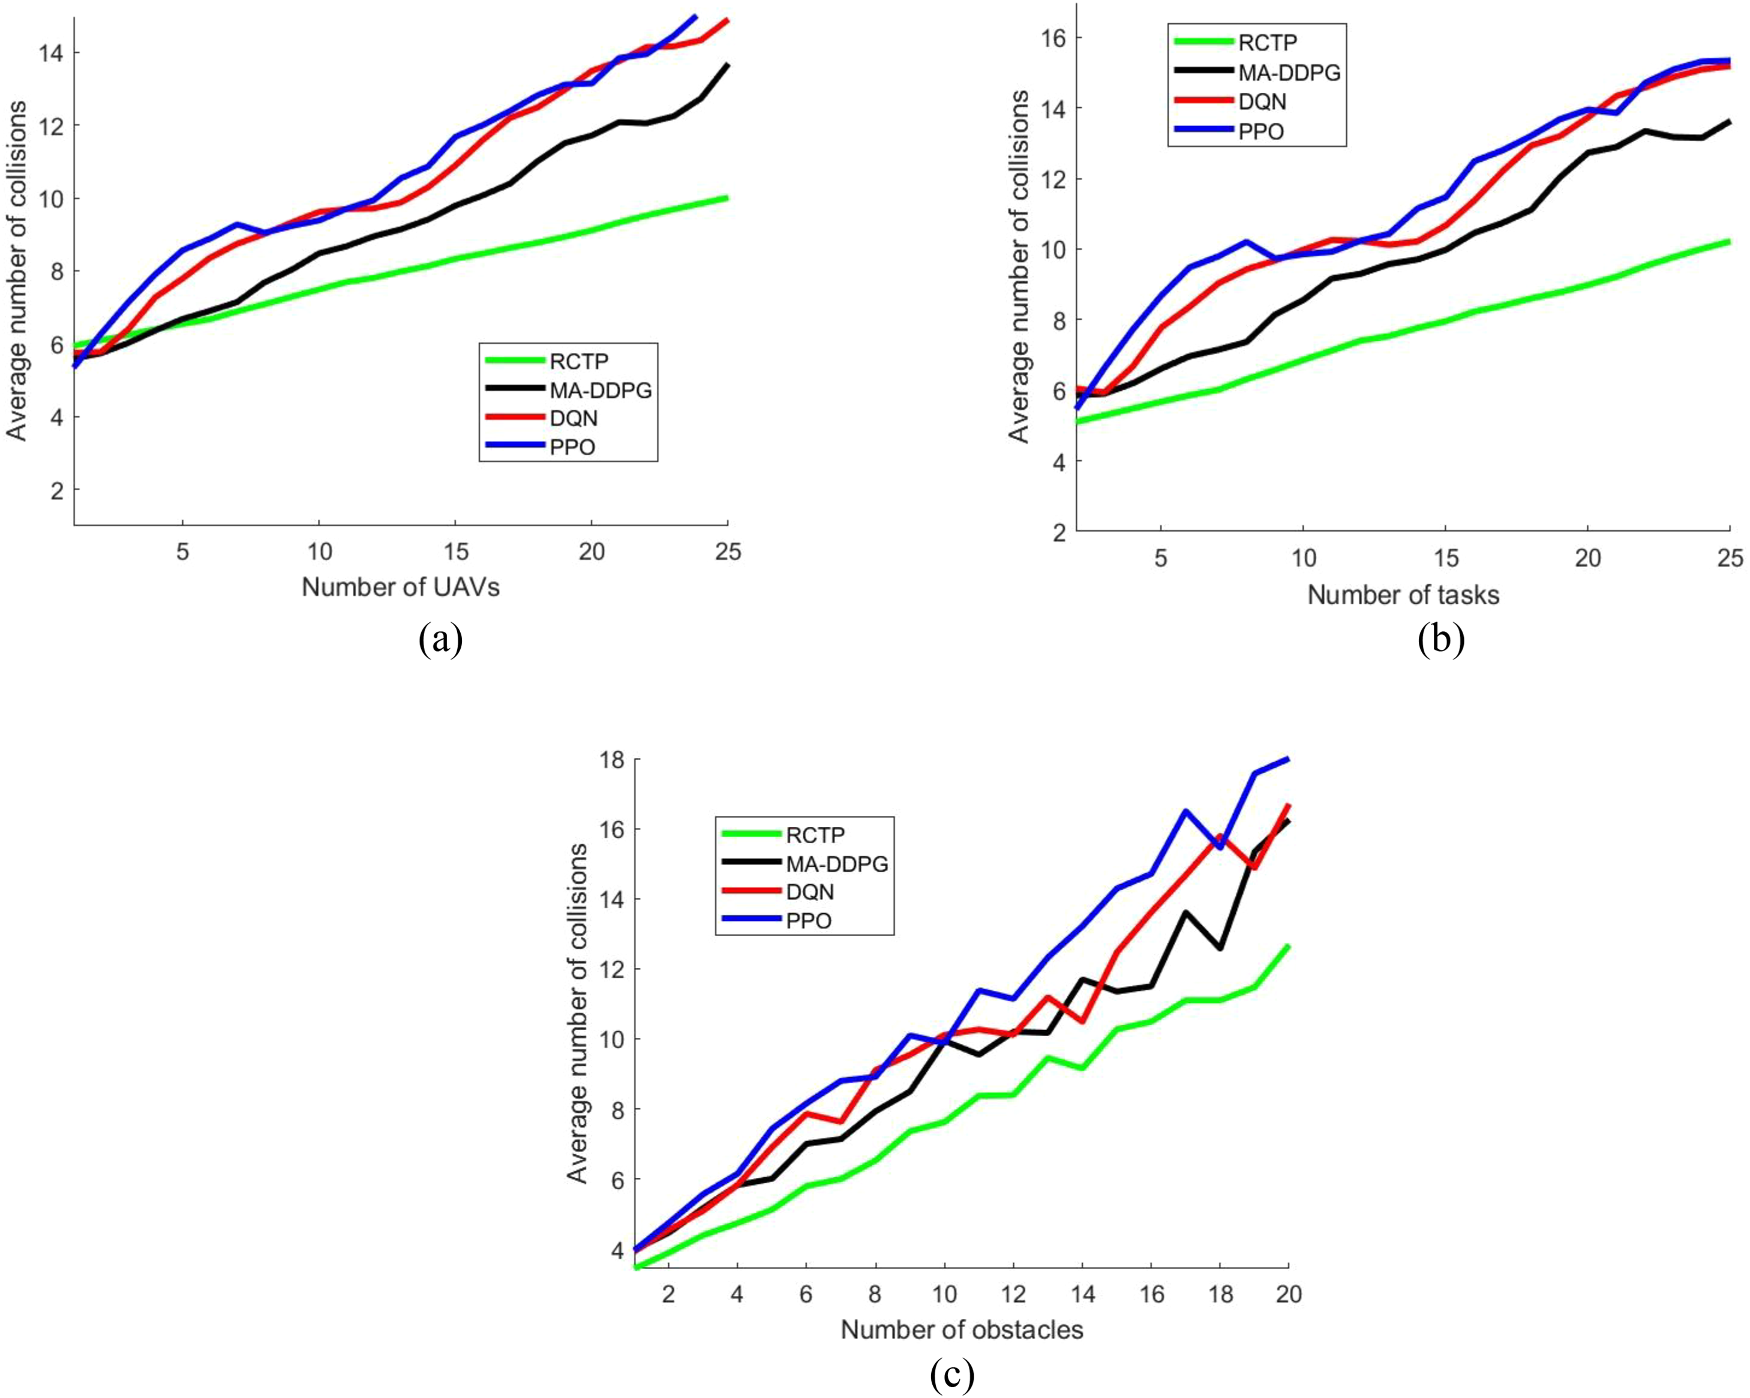
\includegraphics[width=0.82\textwidth]{assets/saras_trajectories.png}
\caption{Non-overlapping multi-UAV flight trajectories across four disaster quadrants}
\label{fig:trajectories}
\end{figure}

\section*{B.2 Coalition Formation and Communication Topology}
Figure \ref{fig:coalition} illustrates the dynamic network topology formed between autonomous aerial agents during sector bidding rounds and victim handover procedures.

\begin{figure}[htbp]
\centering
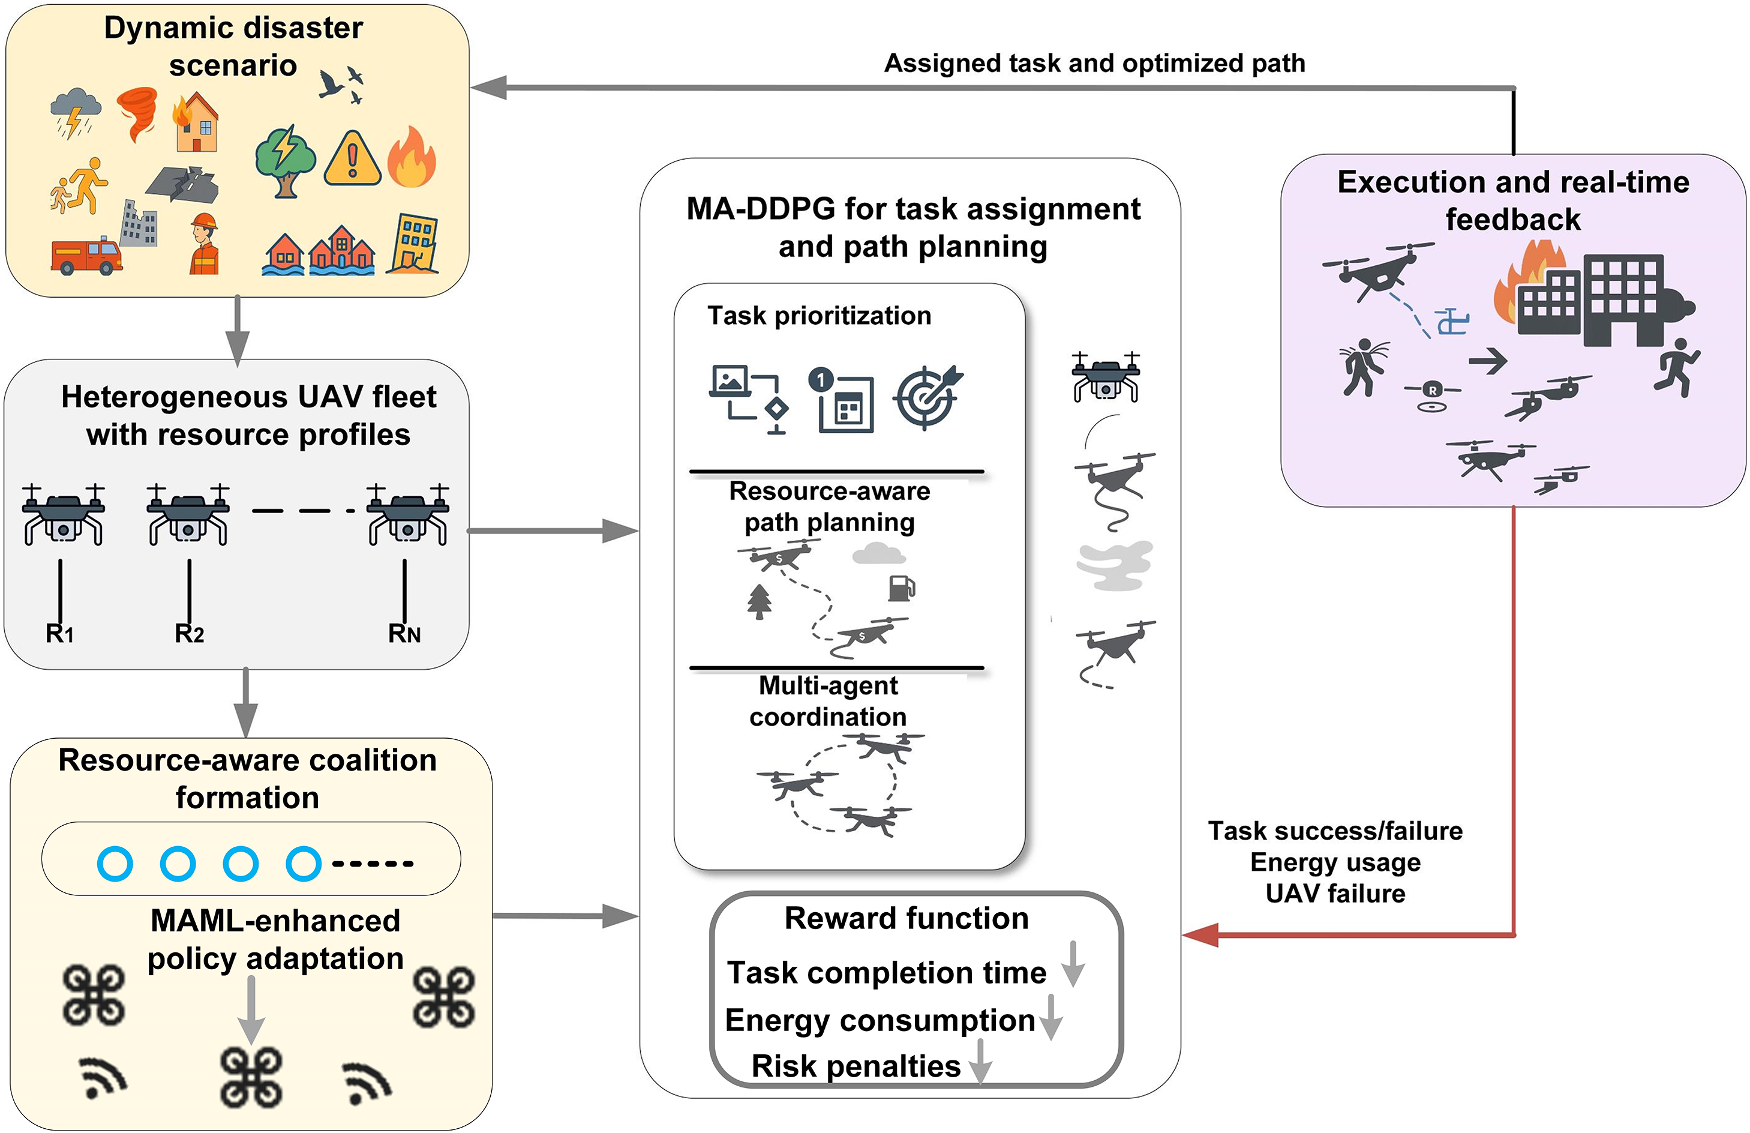
\includegraphics[width=0.82\textwidth]{assets/saras_coalition_formation.png}
\caption{Dynamic peer coalition formation and communication topology during search}
\label{fig:coalition}
\end{figure}

\clearpage
\section*{B.3 Energy Expenditure Distribution}
Figure \ref{fig:fairness} plots the cumulative battery consumption and operational endurance balance across all participating drones, confirming equitable workload allocation.

\begin{figure}[htbp]
\centering
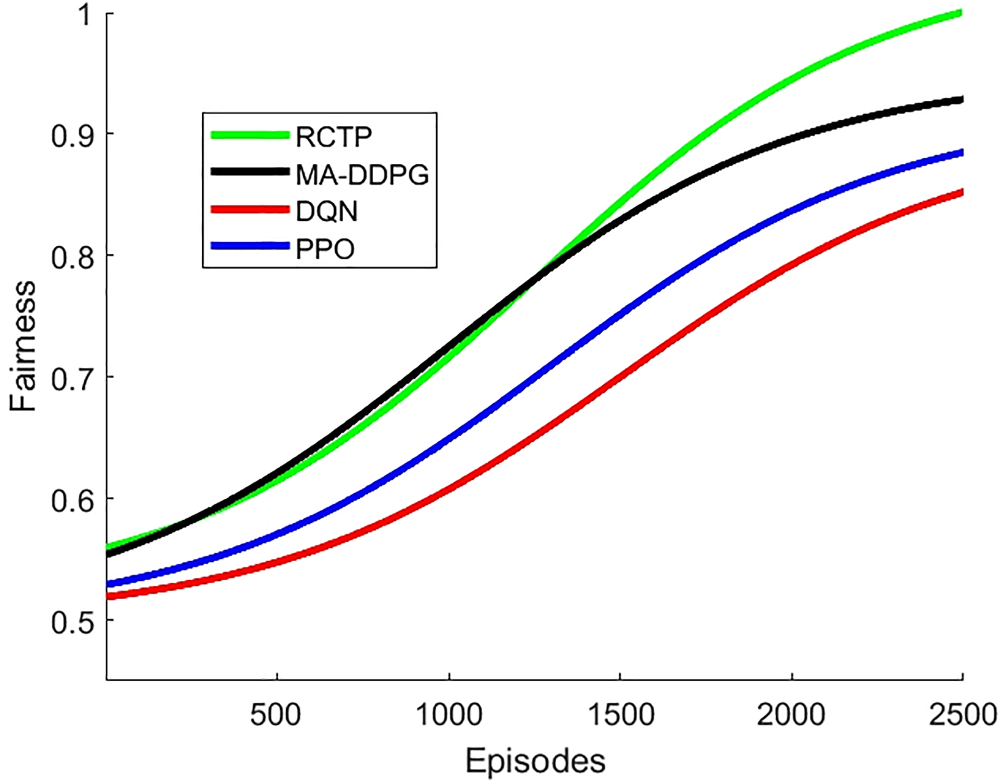
\includegraphics[width=0.85\textwidth]{assets/saras_fairness.png}
\caption{Energy expenditure balance and flight time distribution across the swarm fleet}
\label{fig:fairness}
\end{figure}

\end{spacing}
